\chapter{Learning to play connect four with RL}
\label{ch:connect_four_rl}

The previous chapters introduced the main concepts of \glsfirst{rl} and \glsfirst{marl}.
It was discussed that real-life use cases for \gls{rl} are mostly limited to institutions with a high amount of resources at the moment.
As a possible use case for indie developers, which are small game companies or even individuals, the feasibility of using \gls{rl} as a computer opponent in the simple Python games was studied.
In particular, an open-source Pygame implementation of connect four was converted to a Gym-like environment and common \gls{rl} algorithms were trained in an online manner on it.
This chapter highlights the design decisions of that systems.
All of the documented source code together with annotated Jupyter Notebooks are available on the GitHub repository of this project \citep{github_project}.

%------------------------------------

\section{Connect four and its complexity}
\label{sec:connect_four_rl-harder_then_you_think}

Connect four is a trademarked game first sold in February 1974, although many similar connection board games have been made throughout history.
In connect four, two players compete against each other by dropping player-specific coins into an open slot of a shared board.
This board is seven columns wide and six rows high.
A player drops a coin from the top of a column and it drops to the lowest available row of that column which still has a free spot.
If there is no free spot in a specific column, the coin can not be inserted in that column.
The game is won by the player that can connect four of their pieces in a straight horizontal, vertical or diagonal line.
When to board is full and none of the players has won, the game is a tie. 
A sample game between a rainbow policy and human player is shown in Figure \ref{fig:rainbow_diagonal_win_turn_annotation}, a video of which is also available on YouTube \footnote{\url{https://youtube.com/shorts/DZesQ4GI0hE}}.
It is important to note that connect four is a solved game.
This means that given the first player follows the optimal policy, this player is always guaranteed to win.

The rules of connect four are very simple and with a board of only six by seven, the game seems simple enough.
However, connect four has $4531985219092$ possible boards, which is in the order of $\approx 10^{13}$.
Whilst this is still far less than the game complexity of chess ($\approx 10^{123}$) or Go ($\approx 10^{360}$), it is still significantly larger than the simple rules would suggest.
Since there are so many states, each with up to seven possible actions (free columns), tabular approaches as discussed in section \ref{sec:intro-approaches} are not feasible.
Not only would such a table require significant memory, but it would also take far too long to reach all states at least once.
This further shows how limited tabular methods are.

Whilst a manual feature representation could potentially be determined that lowers the state dimension to a feasible amount, it would require a domain specific approach and would give no value to a general feasibility study.
Because of this, a \glsfirst{drl} approach is taken to learn the connect four game.
This will make it possible to learn directly from the matrix representation of the board shown in the annotations of Figure \ref{fig:intro_rl_cycle}.
Two \glsfirst{dqn} approaches and one Rainbow approach are implemented and trained in a variety of ways, which is discussed in what follows.


\begin{figure}[ht]
    \centering
    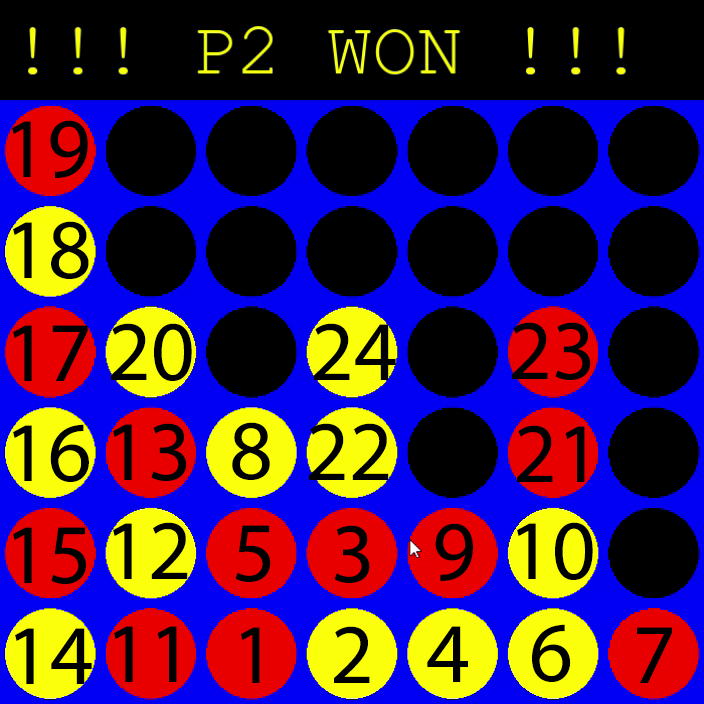
\includegraphics[width=0.7\linewidth]{images/ConnectZero_rainbow_diag_human_win.png}
    \captionsetup{width=0.9\linewidth}
    \captionsetup{justification=centering}
    \caption{Sample connect four game annotated with the time steps at which the coins are placed. Player one is red and is the best-found rainbow policy from the paper notebook 9, player two is yellow and is a human. Player two won with the diagonal coins of 14, 12, 8 and 24.  A video of this game can be found on YouTube (\url{https://youtube.com/shorts/DZesQ4GI0hE}).}
    \label{fig:rainbow_diagonal_win_turn_annotation}
\end{figure}

%------------------------------------

\section{Gym implementation of connect four game environment}
\label{sec:connect_four_rl-gym-environment}


Since this paper aims to study the feasibility of implementing \gls{rl} opponents in simple Python based games, it was chosen to build further upon an existing connect four implementation.
The chosen base implementation is one by \citet{base_connectfour_github} and makes use of the popular Pygame library by \citet{pygame}.
The author's permission of reusing his code was granted after brief communication on LinkedIn.
Some edits were made to this base implementation to make the code more readable and the game UI more informative. 
Since this base game is just a human-play variant of the connect four game, it lacks many of the components required to use it in a \gls{rl} setting such as a reward strategy and more.

As a first step of converting this base Pygame to an environment usable for \gls{marl}, it was converted to a custom Gym environment.
A custom Gym environment should inherit from the Gym class and provide a few specific attributes and functions, a skeleton for this is given in Algorithm \ref{alg:minimal_gym_structure}.
A Gym environment is a class from the popular Gym library by \citet{gym} introduced in section \ref{sec:intro-classical_rl}.
Converting the base Pygame to a Gym environment was straightforward given the many tutorials and documentation available discussing how to create a custom environment.
The conversion process took about four hours, including testing.
This version of the environment is called \texttt{ConnectFourPygameEnvV1} and is available under \texttt{gym\_connect4\_pygame} folder in the Github repository of this project \citep{github_project}. 

The init method supports two render modes, \texttt{terminal} and \texttt{human}.
It also allows for specifying the column and row count of the connect four board, although the default grid of 6x7 is used throughout this paper.
The observation space is specified as a Gym directory consisting of one key called \texttt{board}.
The board in the observation space is a two-dimensional Gym box ($\approx$ 2D array) with integer values between zero and two, including boundaries.
Zero corresponds to an empty space, 1 to the first player's coin and 2 to the second player's coin.
This corresponds to the representation annotated in Figure \ref{fig:intro_rl_cycle}.
The action space is a discrete space specifying an integer that corresponds to the column index a coin should be dropped into.

The step method contains the main logic of a Gym environment as it performs a specified action in the environment and updates the state of the environment.
It also returns a reward, a boolean to specify if the game has ended and an info object.
In this implementation, there is no mechanism in place to reject a player to insert a coin in a full column.
However, attempting to do so keeps the board unaltered and gives the turn to the same player again.
After this, the step function checks for a winning board or tie board to end the game.
If the game is not over, the step function alternates the current player.
The step function makes use of many abstracted functions from the base game, which are not shown in the minimal Gym skeleton of Algorithm \ref{alg:minimal_gym_structure}.

The render method supports a terminal printed render of the board which prints the 2D matrix representation of the board after each step.
It also has support for a human mode which renders the game in a Pygame instance, just like playing the game regularly would do.
The reset and close functions are trivial and are not discussed in detail. 
The experimental notebook 2 gives details on how to work with this V1 of the custom connect four Gym environment \citep{github_project}.
Since the Gym environment doesn't provide any standards on specifying a multi-agent environment, the implementation is custom and does not comply with any specific standard.
In essence, the info object, which is one of the returned values from the step and reset function, gives all the required info for playing a loop in the game.
Since this custom Gym environment is multi-agent but doesn't follow any conventions, it is not supported directly by any \gls{rl} algorithm library and is therefore not used.

\begin{algorithm}
    \caption{Minimal structure of a Gym environment}
    \Comment{Init method should accept a render mode.}
    \Function{\_\_init\_\_(self, render\_mode, ...)}{
        \If{$\var{loss} > \theta_{\mathrm{exp}}$} {
            ... \;
            \Comment{Observation space for the environment: structure of an observation}
            self.observation\_space = gym.spaces.Dict(...)\;
            ...\;
            \Comment{Action space for the environment: structure for an action}
            self.action\_space = gym.spaces.Discrete(...)\;
            ...\;
        }
    }
    \Comment{Reset function to return the environment to its start state.}
    \Function{reset(self, return\_info=False)}{
        ...
        \Return{(observation, info) if return\_info else observation}\;
    }
    \Comment{Step function to perform an action in the environment.}
    \Function{step(self, action: int)}{
        ...\;
        \Comment{Return an observation of the new state, the received reward, a boolean specifying if the environment is finished and an info object containing additional information.}
        \Return{observation, reward, done, info}\;
    }
    \Comment{Render function to visualise the environment.}
    \Function{render(self, mode='terminal')}{
        ...
        
    }
    \Comment{Close function to clean up an environment.}
    \Function{close(self)}{
        ...
    }
    \label{alg:minimal_gym_structure}
\end{algorithm}

%------------------------------------

\section{Petting Zoo implementation of connect four}
\label{sec:connect_four_rl-pettingzoo-environment}

Having implemented the base game as a custom Gym environment in the previous section, it was noted that the Gym library has no direct support or conventions for multi-agent environments.
Because of this, the environment is unlike the other Gym environments, which are all single-agent environments.
This means that it doesn't neatly integrate with existing \gls{rl} algorithm libraries such as Tianshou \citep{tianshou} or Ray RLlib \citep{rllib}.
As this paper is a feasibility study, which includes ease of implementation as a criterion, it was opted to adopt this V1 of the environment to a Petting Zoo environment which is supported by these libraries.
As discussed in section \ref{sec:intro-classical_rl}, Petting Zoo is a commonly used library for \gls{marl} as it provides multi-agent environments in a Gym like fashion.
Converting the custom Gym environment to a Petting Zoo based environment doesn't involve a lot of code changes but did require significant troubleshooting.
This is mostly due to the Petting Zoo documentation not providing instructions on how to implement a custom environment, which the Gym library documentation did do.
However, through studying the source code of simple environments provided by Petting Zoo, such as the Tic-Tac-Toe environment, adopting the custom Gym environment to a Petting Zoo compatible environment took about 15 hours of work.
Most of this time was spent troubleshooting compatibility issues with the Tianshou \gls{rl} algorithm library.

The Petting Zoo variant of the connect four game is provided as \texttt{ConnectFourPygameEnvV2} under the \texttt{gym\_connect4\_pygame} folder in the Github repository of this project \citep{github_project}.  
Most notable changes include inheriting from the Petting Zoo \texttt{AECEnv} class rather than Gym's \texttt{Env} class and wrapping this custom Petting Zoo environment in some common Petting Zoo environment wrappers. 
The observation space is also extended to include an action mask besides the board representation taken straight from the V1 variant of the environment.
This action mask specifies which of the actions from the action space are valid for the current state.
If specified during initialisation, the environment can thus strictly enforce an agent to only use an allowed action for a given state.
Whilst this incorporates some domain knowledge, it can drastically improve the learning speed of the agents.
However, it is still possible to let the agents learn this behaviour by specifying to not use the mask and giving a negative reward for placing a coin in a full column.
Besides this, the observation space and action space should be lists containing a variant of the space for both agents, although these spaces are equal for both agents in the connect four game environment.
Next to this, the \texttt{step} and \texttt{reset} methods no longer return game information such as the state, a done boolean, a reward and an info object.
Rather, Petting Zoo and the libraries that are compatible with it rely on attributes such as \texttt{rewards}, \texttt{dones} and \texttt{infos} to keep track of the game state and an \texttt{observe} function to observe the current state of the environment.
Exact implementation details are not of importance and thus not given in this paper, although the source code is documented and available on GitHub \citep{github_project}.
The final petting zoo environment is over 650 lines of code, compared to the 350 lines of code for the original base game implementation and 450 lines of code for the custom Gym environment (environment V1).  

%------------------------------------

\section{Reward strategy}
\label{sec:connect_four_rl-rewards}

As was discussed in section \ref{sec:marl_opponents}, the target policy of a \gls{marl} problem depends on the reward function, the used discount factor ($\gamma$) and the other agents in the environment.
Whilst the discount factor and agents in the environment can be easily interchanged, the reward strategy has to be implemented in the custom environment.
For the custom Petting Zoo environment, six types of rewards were provided.
The value of each reward can be set during the initialisation of the environment.
The most trivial rewards are those for winning, losing and having a tie game.
To allow for learning not to place a coin in a full column, a (negative) reward for making an invalid move can also be specified.
However, it is noted that the environment can be initialised to use action masks so that the agent can't choose an invalid move, meaning an invalid move would never occur and thus this reward would never be used.

As a means to incentivise longer games, it is also possible to specify a reward for each move made.
Likewise, to incentivise a defensive behaviour by the agent, a reward for what is called a blocking move can also be given.
A move is considered a blocking move if the chosen action by an agent would result in a win for the other agent if the other agent had done that action.
The latter incorporates domain knowledge which guides the agent to learn a good policy.
Whilst this diverges from the purest form of \gls{rl}, it can drastically improve the training time and usability of the policy in terms of human play.
The rewards for making a move and making a blocking move were added incrementally to the environment after it was found that the learned policy using only the other four rewards was very naive.
Chapter \ref{ch:connect_four_eval} discusses the evaluation of the emerged policies and clarifies how different values for these rewards influence the found policies by the agents.


%------------------------------------

\section{Using MLP based deep Q-networks to learn connect four}
\label{sec:connect_four_rl-mlp-dqn}

One of the first very successful \gls{rl} algorithms in learning to play Atari 2600 games at a human level, was a generalisation of the Q-learning algorithm using a \glsfirst{dqn} by \citet{dqn}.
The approach by \citet{dqn} can be seen as a \glsfirst{drl} variant of the popular tabular Q-learning algorithm by \citet{qlearning}.
As discussed in section \ref{sec:intro-approaches}, the difference between tabular methods and \gls{drl} methods is that the first maintains a table of all possible state-action pairs and an expected reward whilst the latter uses \glsfirst{dl} models to map the environment state to an action.
Tabular methods can quickly blow up in dimensionality whilst \gls{drl} can reduce this dimensionality making it possible to solve problems that were not feasible to solve with tabular methods.
As discussed in section \ref{sec:connect_four_rl-harder_then_you_think}, connect four has to many possible states for tabular methods such as Q-learning to be feasible, hence why the \gls{drl} variant \gls{dqn} is used as a first attempt at learning connect four.
More details on how tabular Q-learning works and a convergence proof of the algorithm is given by \citet{qlearning_proof}.

As the name suggests, \gls{dqn} also uses the concept of Q-values just like the Q-learning algorithm but aims to generalise it.
Q-values can be seen as an estimated reward for taking an action ($a$) in a given state ($s$).
These Q-values are the metrics stored in tabular methods for determining and updating the optimal policy.
However, \gls{dqn} doesn't keep track of individual Q-values in a Q-table but rather aims to approximate a Q-function so that the Q-values can be approximated by the Q-function $Q(s, a)$.
In essence, it replaces the Q-table with approximated Q-values in Q-learning by an approximated Q-function.
However, learning that Q-function isn't an easy task, hence why \gls{dl} and more specifically \glspl{ann} come into play.
When using a \gls{dqn}, a \gls{dnn} is used to to approximate the optimal Q-function.

Figure \ref{fig:mlp_dqn} shows one of the \gls{dqn} models that was used for the deep Q-learning of connect four.
This first deep Q-learner is based on a \gls{mlp}.
It consists of three hidden fully connected layers with 128 nodes, all using a ReLu activation function.
The input is the board represented as a 6x7 2D matrix, which corresponds to the state of the environment.
The output is the expected reward for each action if it were taken in that state.
To update this network, a typical loss optimisation is used, in particular, the Adam optimizer proposed by \citet{adam} is used.
The loss function in question is based on the difference in the output of the network with the right-hand side of the Bellman equation given in Equation \ref{eq:bellman}.
Since this target policy makes use of the maximum action $a'$  in the new state $s'$ upon taking an action $a$ in the current state $s$, it differs from the behaviour policy which might use something like epsilon-greedy as well.
Since these two policies are not equal, deep Q-learning is an off-policy approach, just like regular Q-learning, as was discussed in section \ref{sec:intro-approaches}.


\begin{equation}
q_*(s, a) = E[ R_{t+1} + \gamma \max_{a'} q_* (s', a') ]
\label{eq:bellman}
\end{equation}

More technical details on the working of deep Q-learning by using a \gls{dqn} can be found in the paper by \citet{dqn} which first proposed this algorithm.
One of the attractive properties of using the custom Petting Zoo environment is that it directly integrates with the Tianshou library by \citet{tianshou}.
This Tianshou library provides an off-policy learner and a \gls{dqn} policy, which allows for using \gls{dqn} just by specifying which network architecture to use.
This makes the implementation of this rather complex algorithm for our custom connect four Petting Zoo environment extremely simple.
All that has to be done is providing the Pytorch model of the \gls{mlp} based \gls{dqn} shown in Figure \ref{fig:mlp_dqn}.
More implementation details and the chosen parameters for some of Tianshou functions can be found in the paper notebooks 3, 4 and 5 available on the GitHub repository of this project \citep{github_project}.

\begin{figure}[ht]
    \centering
    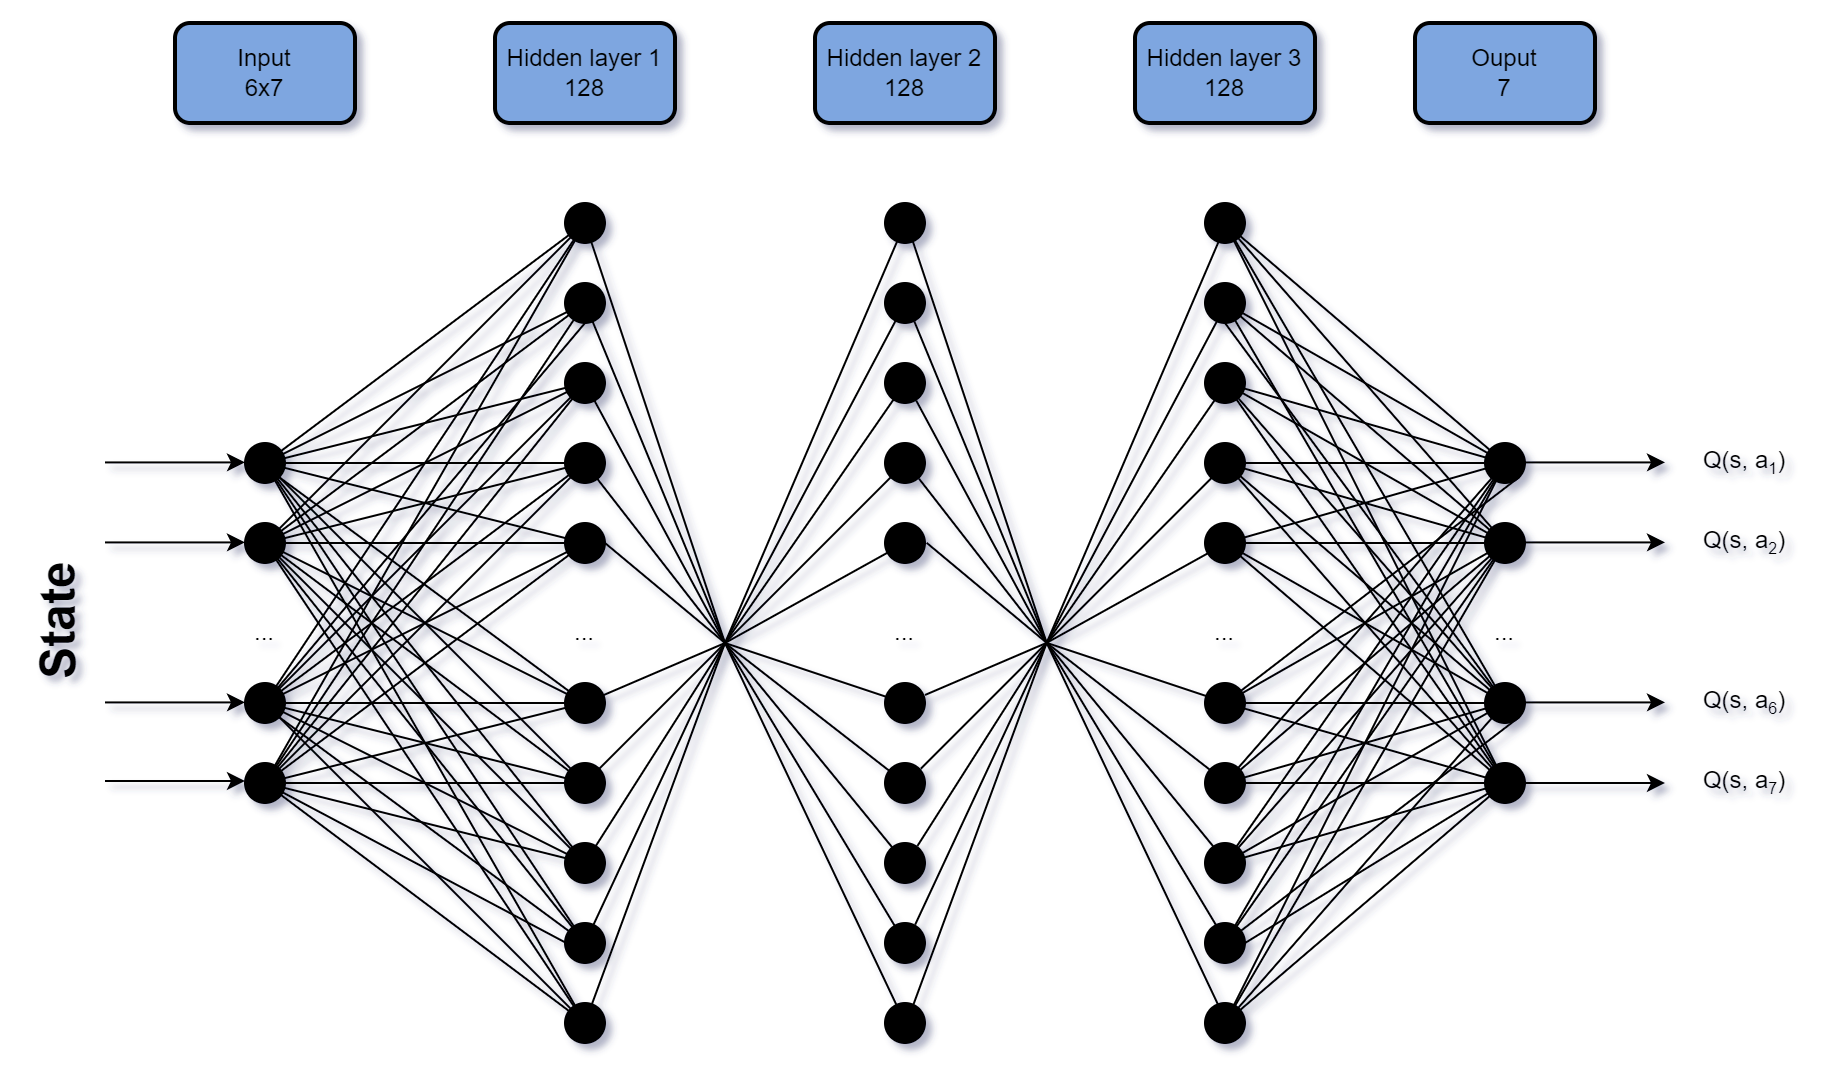
\includegraphics[width=1\linewidth]{images/mlp_dqn.png}
    \captionsetup{width=0.9\linewidth}
    \captionsetup{justification=centering}
    \caption{\gls{mlp} based \gls{dqn} architecture used for Deep Q-Learning.}
    \label{fig:mlp_dqn}
\end{figure}

%------------------------------------

\section{Using CNN based deep Q-networks to learn connect four}
\label{sec:connect_four_rl-cnn-dqn}

The \gls{mlp} based \gls{dqn} proposed in section \ref{sec:connect_four_rl-mlp-dqn} is sophisticated enough that it likely won't be a factor in making learning of the connect four game impossible.
However, there is a more logical architecture to be used.
This more logical architecture revolves around using a convolution layer, forming a type of \gls{cnn}.
Convolution layers are often used for image processing and an in depth explanation of this layer is given by \citet{cnn_explained}.

Intuitively, the 2-dimensional convolutional layer used for the \gls{dqn} goes over the input 2D board representation with a 4x4 kernel.
This kernel consists of a 4x4 grid of weights that have to be learned.
These weights are used to perform a convolution of the 4x4 grid to a singular value.
This kernel moves over the 2D board matrix in a left to right, top to bottom manner, moving by one element each time.
This reduces the initial board input of a 6x7 2d matrix to a 2d matrix of 3x4.
The kernel uses the same weights for the whole board in a single filter.
This process is visualised in Figure \ref{fig:cnn_kernel_explained}.

\begin{figure}[ht]
    \centering
    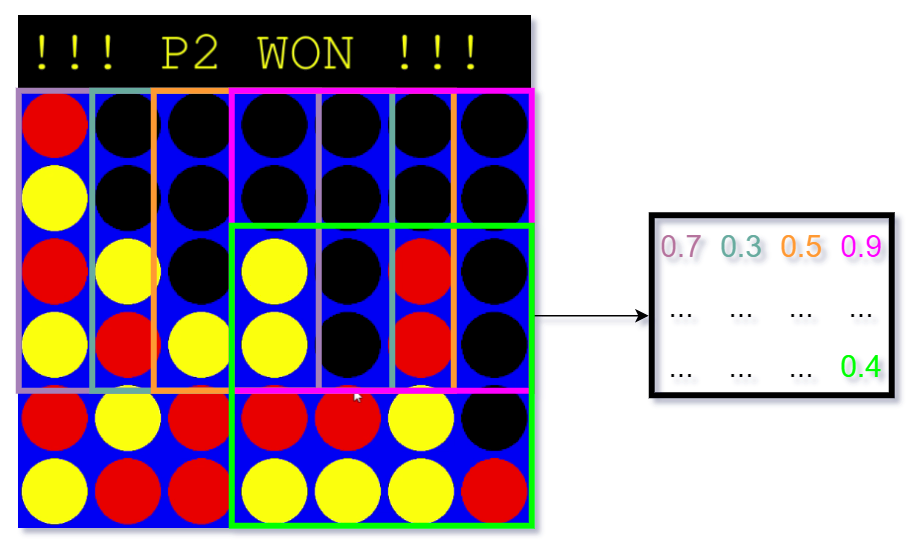
\includegraphics[width=0.7\linewidth]{images/cnn_explained.png}
    \captionsetup{width=0.9\linewidth}
    \captionsetup{justification=centering}
    \caption{Single convolutional filter for a 4x4 kernel with stride one.}
    \label{fig:cnn_kernel_explained}
\end{figure}

Whilst only one such filter would greatly reduce the input dimension, a lot of information would be lost.
At least both diagonal lines, four horizontal lines and four vertical lines should be recognisable since these form a win or a loss condition. 
Whilst it would be possible to learn these conditions with fewer filters, it is reasoned at least 10 or even 20 filters should be available to recognize all win and loss conditions.
Since the computational overhead of providing more filters isn't drastic and it can give better performance by allowing to learn more than just the win conditions, it was opted to create 64 filters.
This results in a final output dimension of 3x4x64 for the convolutional layer.
After this convolutional layer, the output is flattened and two fully connected layers of size 128 are provided before going to the output layer of the network.
In essence, the hidden layer 1 shown in Figure \ref{fig:mlp_dqn} is replaced by 64 filters of the CNN layer visualised in figure \ref{fig:cnn_kernel_explained}.
The implementation of this \gls{cnn} based \gls{dqn} is performed in paper notebook 6 which is available in the GitHub repository of this project \citep{github_project}.


%------------------------------------

\section{Using CNN based Rainbow to learn connect four}
\label{sec:connect_four_rl-rainbow}

Whilst \gls{dqn} has proven to be very powerful at learning single-agent Atari 2600 games, there are some issues with \gls{dqn}.
Many extensions have been proposed to solve one or more of these issues, but they fail to solve all of them or even introduce new ones, as discussed by \citet{rainbow}.
To solve this, \citet{rainbow} proposed a \gls{rl} algorithm that combines all of the strong points of six different \gls{dqn} extensions into a single \gls{rl} algorithm.
This resulted in the best final performance based on the median human-normalized score for 57 Atari 2600 games and required fewer sample frames to do so than any of the individual extensions.
The exact details on the Rainbow algorithm can be found in the \citet{rainbow} paper.
One of the nice things about using the Tianshou library by \citet{tianshou} is the fact that many of these state-of-the-art and complex algorithms are implemented already and can be set up with relatively few lines of code and only a high-level understanding of the algorithm.

The Rainbow algorithm is implemented to use the same convolutional layer of the \gls{cnn} based \gls{dqn} from section \ref{sec:connect_four_rl-cnn-dqn}.
This layer can be seen as a feature extraction layer.
Subsequent layers are adapted from the original Rainbow paper by \citet{rainbow}, where noisy linear layers are used together with an epsilon-decay.
Normally, the algorithm only uses one of these two to make the agents exploratory, but to combat the low amount of training samples due to limited computational power and to incentivise keeping an exploratory behaviour, they are used together for this project.
The rainbow algorithm also makes use of the duelling property described by \citet{dueling} as it should aid in learning a good policy for this \gls{marl} connect four environment.
The implementation of the Rainbow algorithm is further described in the paper notebook 9 on the GitHub repository of this project \citep{github_project}.

%------------------------------------

\section{Using mini-max as a rule-based opponent}
\label{sec:connect_four_rl-minimax_opponent}

Finally, a mini-max based algorithm is implemented to function as a connect four player.
Mini-max is a game tree searching algorithm that can make use of alpha-beta pruning to limit the number of trees to visit.
Intuitively the mini-max algorithm alternates in maximising (current player's optimal strategy) and minimising (opponent's player optimal strategy) the chosen action based on a given score that is returned at the end of the recursive process.
Since it is computationally too hard to do this for the full depth of the game tree, it is only done for a specified depth.
The recursive loop stops once the desired depth is reached or the game is terminated.
When the desired depth is reached, the score of that final state is determined by the number of consecutive coins present on the board for both agents.
If the tree results in a win, the maximum score is returned and if it results in a loss, the minimum score is returned.
A tie is given a score of 0.
Normally, the deeper the search depth, the stronger the policy of the mini-max agent.


However, a mini-max agent does not form a pleasant opponent, since even the simplest mini-max agent with depth 1 will always block a winning move by design.
Thus, to win against the smallest depth mini-max agent, a scenario has to be created where two possible winning moves have emerged.
This ensures that even when the mini-max bot blocks one of them, the game can still be won by playing the other.
This is a rather hard scenario to obtain, and as the depth of the mini-max agent increases, the mini-max agent can anticipate this as well, making it near impossible to beat as a human, even with a depth of only 3.
An ideal bot will sometimes fail to see a potential win for the opponent, as humans would also do.
The mini-max implementation used in this project is based on a mini-max connect four agent by \citet{minimax_base}.
\Citet{minimax_explained} explain the mini-max algorithm in more depth.


Since mini-max uses a fixed policy and doesn't learn from the algorithm, playing against mini-max can be seen as single-agent \gls{rl} as described in section \ref{sec:marl-vs_single}.
However, this mini-max agent has been made available as a Tianshou \texttt{BasePolicy} object so that it can be used in the same multi-agent training pipeline that is used for self-play.
The idea behind playing against a mini-max agent is to provide a strong opponent to learn from for the \gls{rl} agents.
As it is assumed that increasing the depth of the mini-max agent will increase its policy's strength, changing this depth allows for creating a league-based training setting as described in \ref{sec:marl_opponents}.
The best scoring \gls{rl} agent for each of these iterations in the league based training loop would then be incrementally better over the previous iteration.
This would ideally provide varying difficulties for the connect four \gls{rl} bot.
Paper notebook 11 describes this in more depth and is available on the GitHub repository of this project \citep{github_project}.